% This is a LaTeX source file with extensive commentary for learning LaTeX.
% It is a modified version of a file due to Dr. Kevin P. Lee, now at Chicago's Simeon Career Academy High School.

% You can used this file as a LaTeX template.
%Copy this file and make any adaptations which you need.
%Consult a LaTeX guide for further information about TeX and LaTeX.

% The Very Basics:

%	1. Anything on a line after the character ''%'' appears in red and is ignored 
%		by LaTeX. Thus you can delete any line beginning with ''%" and nothing about the output
%		will change (although these comments are often very helpful).

%	2. The backslash "\" precedes commands.

%	3. Command arguments are enclosed by braces "{}".

%	4. All LaTex source files (this is a source file; it has the suffix .tex) begin with 
%		the line \documentclass{"class"}, where "class" specifies a particular
%		type of formatting.

%	5. There are two main parts of a source file:
%		a) Everything after \documentclass but before \begin{document} is
%			called the "preamble" -- it defines properties of your document.

%		b) The text of your document occurs between the commands
%			\begin{document} and the very last command \end{document}.


%\documentclass{article}	% This tells LaTeX to format the content into the style of an article.
                                        
%\documentclass[11pt]{article}		% You can include some options within the 
							% square brackets. These options will affect 
                                        			% the formatting of the entire document. The
                                      			% option here selects for a type size of
                                        			% 11 points. This line is currently ignored
                                       			% by LaTeX. To use this option, add a "%" at
							% the beginning of the other \documentclass
							% command and delete the ''%'' at the
							% beginning of this line. Similar instructions
							% apply to each of the following lines.

\documentclass[12pt]{article}          % You can also select a type size of 12 points.

%\documentclass[legalpaper]{article}	% This causes the output to be formatted
								% onto a legal-sized document.

%\documentclass[landscape]{article}	% This causes the output to be formatted
								% ''sideways''.

%\documentclass[twocolumn]{article}	% You can specify two columns on each page.

%\documentclass[leqno]{article}	% The ''leqno'' option specifies that equation 
                                        			% numbers will be placed on the left instead of 
                                        			% the right.

%\documentclass[fleqn]{article}         % Instead of centering displayed formulas,
							% formulas will be aligned on the left.

%\documentclass{report}			% This line will cause the content to be formatted 
							% into a report. The report class is better for 
							% longer documents.
                                        
%\documentclass{book}			% The book class is best for very long documents.

% You can combine various document options and classes. For instance, suppose that
% you want a book written in 12 point typeface, two columns, and with equations
% aligned on the left. Then you should specify:

%\documentclass[12pt,twocolumn,fleqn]{book}

%%%%%%%%%%%%%%%%%%%%%%%%%%%%%%%%%%%%%%%%%%%%%%%%%%%%%%%%%%%%%%%%%%%%%%%%%%%%%%%%

% Now we begin the PREAMBLE:

% The \usepackage command will read additional files which will either affect the
% formatting of the entire document or allow you to use additional commands. 
% Some files are standard. Others can be downloaded from the web. Typically,
% these extra files will end in the suffix ''.sty''. So the command
% ''\usepackage{example}'' will cause LaTeX to read the file ''example.sty''.

% These next several \usepackage commands will cause LaTeX to use different fonts.
% Notice that all of these lines will be ignored by LaTeX unless you delete one of
% the  ''%'' characters at the beginning of a line.

%\usepackage{times}	% The package ''times'' will cause LaTeX to use the
					% Times font throughout most of your document.

%\usepackage{palatino}		% Use Palatino.
%\usepackage{bookman}		% Use Bookman.
%\usepackage{newcent}		% Use New Century Schoolbook.
%\usepackage{garamond}	% Use Garamond.

% These next few commands will allow you to use some additional mathematical
% typesetting commands.

\usepackage{amsmath}		% The ''amsmath'' package will allow you to use useful 
						% commands contained within the AMS-LaTeX package.
						% (AMS is the American Mathematical Society.)
					
\usepackage{amssymb}		% The ''amssymb'' package will allow you to use 
						% additional mathematical symbols.
						
\usepackage{amsthm}		% The ''amsthm'' package contains commands
						% for formatting mathematical theorems and 
						% statements.

% These next packages allow you to include graphics within a LaTeX document.
% Please read the available documentation before trying to use these packages.
% They will not be loaded due to the ''%'' characters at the beginning of the lines.
%  To use these packages, delete the ''%'' characters.

\usepackage{graphicx}

\usepackage{setspace}		% The ``setspace'' package contains new 
						% commands that will facilitate doublespacing 
						% a document. Make sure that you have the file 
 						% ''setspace.sty'' contained in the same folder as 
						% the source file.
                                        
%\doublespacing			% The ''\doublespacing'' command is available only if
						% ''\usepackage{setspace}'' is in the document. This 
						% causes the document to be double-spaced (surprise!).
                                        
\onehalfspacing			% Alternatively, one can use ''\onehalfspacing'' with 
						% the ''setspace'' package.

% If you do not want to use the ''setspace'' package, you could use the command
% ''\baselinestretch{2}'' or ''\baselinestretch{1.5}'' in your document. In some
% situations though, this produces bad results.

\usepackage[top=1in,bottom=1in,left=1in,right=1in]{geometry}	   % The ``geometry" package
					% allows you to specify the margins of the document. For example, the
					% options indicated in the square brackets set all margins except the left 
					% to 1" and the left margin at 1.25".

%%%%%%%%%%%%%%%%%%%%%%%%%%%%%%%%%%%%%%%%%%%%%%%%%%%%%%%%%%%%%%%%%%%%%%%%%%%%%%%%

% Now we begin the BODY OF YOUR DOCUMENT:


\begin{document}	% All LaTeX files contain the command ''\begin{document}''. 
				% There is a corresponding ''\end{document}'' command
				% at the end.

% Next we'll give basic titling information to LaTeX:

\title{MODELING AN ARMS RACE}		% The title of the document.
								% The ~ symbol forces a space; try removing it to see 
								% what happens.


\author{Jonathan Ledesma, Khoa Nguyen, Alishan Premani}					% The author


\date{\today}				% This date-stamps your paper automatically. If you want to 
						% specify a fixed date, you may do so between the braces.
						% If you don't want a date to appear, type ''\date{}''.

% Creating the title section:

\maketitle		% This command creates the appropriate header. It may alternatively
			% create a title page. This will depend on whether you have selected  
 			% ''report'', ''book", or ''article'' in the ''\documentclass'' command above.
			
%pull, add commit, push

\begin{center}
{\large \bfseries Introduction} % Major section
\end{center}

Every country is concerned about its national security. Maintaining an inventory of weaponry is one of the priorities in defense, but how a country does it depends on not only its own inventory, but also on other factors, such as technological advances, other countries' inventories of weaponry, and the tension between them. In this paper we seek to create a simple model of differential equations to investigate the change in weaponry of two countries in relation to one another, and to improve our model by factoring another variable into our equations. Then we apply our model to the Cold War between the United States and the USSR where there was an arms race between the two countries. Due to limited time and resources, as well as techniques and skills in solving differential equations, our model has a lot of room for improvement, considering the number of variables not present in our equations.

\newpage

% Khoa
\section{Assumptions}
We define the following variables:
\begin{itemize}
\item $x(t) \ge 0$ is the amount of weaponry that country X has at time $t$,
\item $y(t) \ge 0$ is the amount of weaponry that country Y has at time $t$,
\item $a \ge 0$ is the coefficient of new weapon production of country X,
\item $b \ge 0$ is the coefficient of new weapon production of country Y.
\end{itemize}
We restrict this model to a specific time interval in which $a$ and $b$ stay constant, even though in a real-world situation, the production rates might fluctuate.

%JONATHAN LEDESMA
\section{Simple Model}	
The simple model looks at the production of weaponry for each country solely dependent on the other country's amount of weapons. Without considering other factors, a country will only look at the other country's rate of production and number of weapons at time $t$. The simple model can be defined as:
$$\begin{cases}
\frac{dx}{dt} = & ay \label{eq:changeInsimpleX} \\
\frac{dy}{dt} = & bx \label{eq:changeInsimpleY}.
\end{cases}$$
In this model $a$ and $b$ are the rates of production and both $x$ and $y$ are the amount of weapons the other country holds. From this system of equations we create the matrix, 
\[\begin{bmatrix}
    0 & a\\ 
    b & 0
\end{bmatrix}.\]
From this matrix we obtain the characteristic polynomial and our eigenvalues, 
\begin{align}
\lambda=\pm \sqrt{ab}.
\end{align}
Thus we get the general solution for $y$, 
\begin{align}
{y}(t)=k_1e^{\sqrt{ab}t}+k_2e^{-\sqrt{ab}t}.
\end{align}
Finally plugging in our general solution for $y$ into $\frac{dx}{dt}$ we obtain the general solution for $x$,
 \begin{align}
{x}(t)=\sqrt{\frac{a}{b}}(k_1e^{\sqrt{ab}t}-k_2e^{-\sqrt{ab}t}).
\end{align}
We now plug in the initial conditions $x(0)=235$ and $y(0)=1$ with rates of production $a=\frac{10}{23}$ and $b=\frac{14}{25}$. Section \ref{coldwar} will explain the choice of this particular initial condition and these parameters. Solving for the constants $k_1$ and $k_2$, we get $k_1\approx104$ and $k_2\approx-103$. Thus the solution for this initial value problem is:
$$\begin{cases}
{x}(t)=\sqrt{\frac{125}{161}}(104e^{\sqrt{\frac{28}{115}}t}+103e^{-\sqrt{\frac{28}{115}}t})\\
{y}(t)=104e^{\sqrt{\frac{28}{115}}t}-103e^{-\sqrt{\frac{28}{115}}t}.
\end{cases}$$
In the next section, we observe a model that accounts for more factors. 	

%Alishan
\section{A More Realistic Model}
Now we consider the situation where both countries decide to update their inventory of weaponry due to new technological advances and expired old weapons. 
Therefore, we define additional parameters in the differential equations:
$$\begin{cases}
\frac{dx}{dt} = & ay - cx \label{eq:changeInX} \\
\frac{dy}{dt} = & bx - dy \label{eq:changeInY}	
\end{cases}$$
where $c \ge 0$ and $d \ge 0$ are constant coefficients of the destruction of old weapons in countries X and Y, respectively.  \\
We can solve this system of differential equations by constructing a coefficient matrix $M$ as follows
\[
\bold{Y}(t) = 
 \begin{bmatrix}
	dx/dt \\ dy/dt
 \end{bmatrix}
= \begin{bmatrix}
    -c & a\\ 
    b & -d
  \end{bmatrix}
  \begin{bmatrix}
    x \\ y
  \end{bmatrix}, \quad
  M=
  \begin{bmatrix}
    -c & a\\ 
    b & -d
  \end{bmatrix}.
  \]
where $c \ge 0$ and $d \ge 0$ are constant coefficients of the destruction of expired weapons in countries X and Y, respectively.
Our equilibrium solution is (0,0), when both the countries' amounts of weaponry are zero. When $Det(M) = cd - ab$, we have infinitely many equilibrium points along a straight line. 
Note that the trace $Tr(M)\le0$ because of our assumptions that $c \ge 0$ and $d \ge 0$.\\
\\Our characteristic polynomial is $\lambda^2 + (d+c)\lambda + cd - ab$. We use Maple to compute the eigenvalues and eigenvectors, yielding
	\begin{align}
	\lambda_1 = -\frac{1}{2}d - \frac{1}{2}c + \frac{1}{2}\sqrt{4ab -2cd + c^2 + d^2}, \quad \vec{v}_1 = 
	\begin{bmatrix}
	\frac{a}{\lambda_1}\\
	1
	\end{bmatrix},\\
	\lambda_2 = -\frac{1}{2}d - \frac{1}{2}c - \frac{1}{2}\sqrt{4ab -2cd + c^2 + d^2}, \quad \vec{v}_2 = 
	\begin{bmatrix}
	\frac{a}{\lambda_2}\\
	1
	\end{bmatrix}.
	\end{align}	
We now discuss the different possible cases which can occur during the arms race by using the above eigenvalues and eigenvectors. These cases are in terms of various combinations of rates of production and destruction of weaponry and potential relations between the two countries.


\subsection{Case 1 - Two Real Distinct Eigenvalues}

We rewrite the equation for $\lambda$ as follows
	\begin{align} \label{lambda}
	\lambda & = -\frac{1}{2}(d + c) \pm \frac{1}{2}\sqrt{4ab -2cd + c^2 + d^2}.
	\end{align}
Since $Tr(M) \le 0$, we have 
	\begin{itemize}
	\item a saddle when $Det(M) = cd-ab < 0$, implying that $cd<ab$. This is when one country has higher and lower production and destruction rates respectively than the other, leading it to win the race.
	
	\item a sink when $Det(M) = cd-ab > 0$, implying that $cd>ab$. This is when the product of both the countries' rates of destruction of weapons is greater than the product of their rates of production. 
	This might happen when, for instance, both countries decide to either end the arms race for whatever reason, or shift the race to another advanced class of new weaponry.
	
	\end{itemize}
To have two real distinct eigenvalues, we need the discriminant in equation \eqref{lambda} to be greater than zero
	\begin{align} \label{discGreaterThanZero}
	4ab -2cd + c^2 + d^2 & > 0,
	\end{align}
which implies that $4ab + c^2 + d^2 > 2cd$. 

We break this down further into separate cases.
	\begin{enumerate}
 		\item The first sub-case is where $c = d$, which gives us $4ab > 0$. This implies that $a \ne 0$ and $b \ne 0$ for the inequality to hold true. Therefore, when both countries destroy their own arms at equal rates, they both must have non-zero production rates for arms. This is because we assume both countries to be competing to have more arms than the other. So if both countries destroy their weapons at equal rates, then these countries must produce at least some weapons in order to stay competitive.
		\item The second sub-case is where $c \ne d$ (both countries destroy their weapons at different rates), which implies that $c^2 + d^2 > 2cd$. Thus, it must hold true that $a\ge 0$ and $b \ge 0$, which is our assumption. We can infer that in this case, we can expect both countries' rates of production to be flexible in that either one or both of them may not be producing any weapons at any given time. Since it must be true that one of the countries rates of destruction is less than the others' when $c \ne d$, then that country would not be as worried as the other country to produce more weapons to stay competitive.
	\end{enumerate}
The general solution for this case is 
	\begin{align}
	\bold{Y}(t) = k_1 e^{\lambda_1 t}\vec{v}_1 + k_2 e^{\lambda_2 t}\vec{v}_2,
	\end{align}
where $k_1$ and $k_2$ are constants depending on the initial condition.

\subsection{Case 2 - Repeated Eigenvalues}

To have repeated eigenvalues, we must have our eigenvalue be in the form $\lambda_r = -\frac{1}{2}(d + c)$ from equation \eqref{lambda}. Note that we can have only non-positive repeated eigenvalues since $a\ge0$ and $b\ge0$.
We can only have a sink, where both countries tend to have a net decrease in the amount of weaponry they possess.

The discriminant in equation \eqref{lambda} must be equal to zero
	\begin{align} \label{disEqualToZero}
	4ab -2cd + c^2 + d^2 & = 0,
	\end{align}
which implies that $4ab + c^2 + d^2 = 2cd$. 
Again, we break this into further branches.
	\begin{enumerate}
 		\item The first case is where $c = d$, which implies that $c^2 + d^2 = 2cd$. Thus at least one of $a$ and $b$ must be zero, which means that at least one country's production must be zero. Since both countries have a net decrease in the amount of weaponry they have, it is logical to predict at least one country to not produce any weaponry at all.
		\item The second sub-case where either $c = 0$ or $d = 0$ but not both, since $c \ne d$. For example, if $c = 0$, then $4ab = -d^2$, which is not possible because of our assumptions. Therefore, it is not possible to have this case because both countries must have a non-zero rate of destruction, since there is a net decrease in their respective amounts of weaponry, as noted earlier.
	\end{enumerate}
The general solution for this case is 
	\begin{align}
	\bold{Y}(t) = e^{\lambda_r t}
	\left[ \begin{matrix}
	x_0 \\ y_0 
	\end{matrix}\right]
	+ te^{\lambda_r t}
	\left[\begin{matrix}
	-c - \lambda_r & a \\
	b & -d - \lambda_r 
	\end{matrix}\right]
	\left[ \begin{matrix}
	x_0 \\ y_0 
	\end{matrix}\right],
	\end{align}
where $x_0$ and $y_0$ are the initial conditions.	
	
\subsection{Case 3 - Complex Eigenvalues}

For complex eigenvalues to occur, we must have the discriminant to be less than zero
	\begin{align} \label{disLessThanZero}
	4ab -2cd + c^2 + d^2 < 0,
	\end{align}
implying that $4ab + (c - d)^2 < 0$. However, due to our assumptions that $a, b, c, d \ge 0$, this can never occur. 

\section{Case Study: Cold War}\label{coldwar}
We consider the arms race between the United States and the USSR during the Cold War between 1949 and 1979. Due to limited time and resources, we define the term ``weaponry" in this case to only include nuclear warheads. We also exclude other external factors such as internal political conflicts in each country, current wars at the time, and treaties, that would effect the production and destruction rates of weaponry in each country.\\
\\Let the United States be our country X and the USSR be our country Y in the above models. Then $x(t)$ represents the amount of warheads the United States had and $y(t)$ represents the amount of warheads the USSR had.\\
\\The number of stockpiled warheads of the United States and the USSR in this period of time is given and illustrated by the following table and graph:\\
\\
\begin{center}
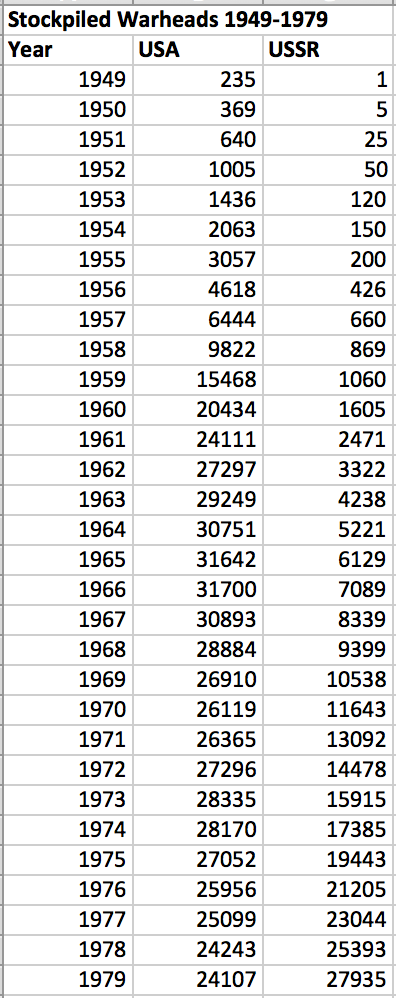
\includegraphics[width=0.3\linewidth]{warheads-table}
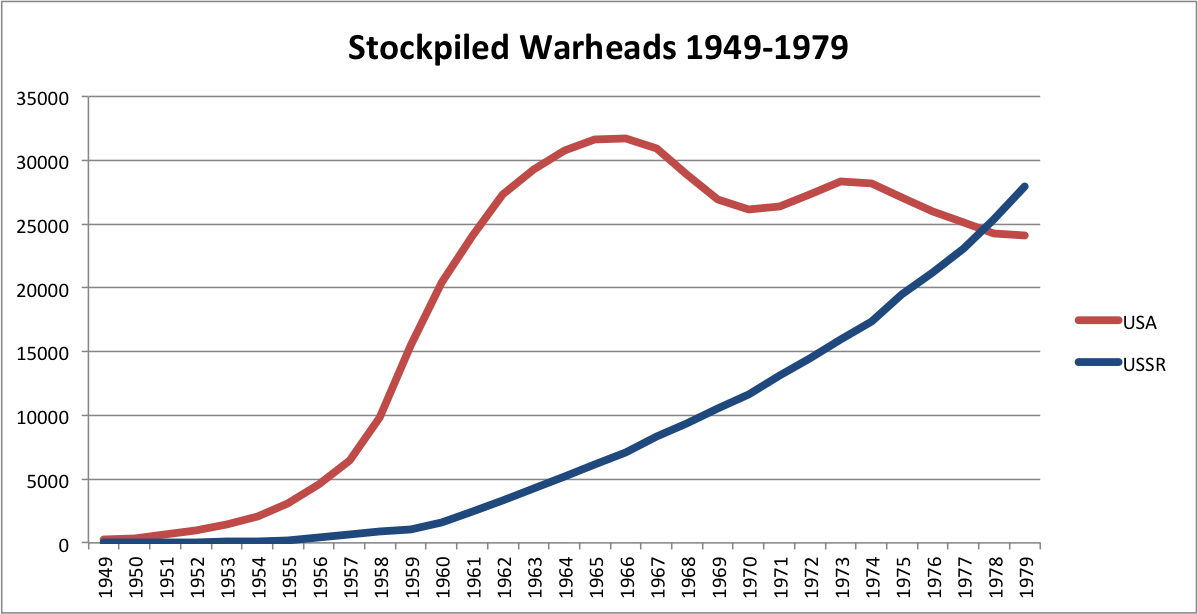
\includegraphics[width=0.8\linewidth]{warheads}
\end{center}
Through a lot of trial-and-error, we find that $a = 10/23$, $b=14/25$, $c=11/25$, and $d = 1/5$ give the best approximation of $x(t)$ and $y(t)$ given the actual data. The graphs of theoretical $x(t)$ and $y(t)$ versus $t$ are below, where the red curve is $x(t)$ for the United States, the blue curve is $y(t)$ for the USSR, and the initial condition is $x(0) = 235$ and $y(0) = 1$:\\
\\
\begin{center}
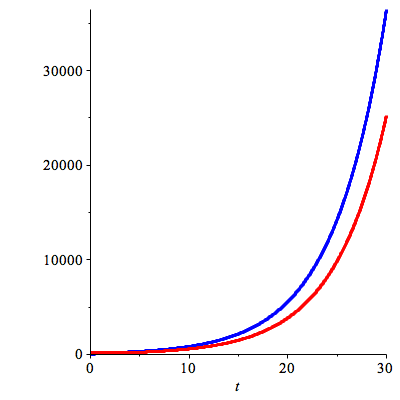
\includegraphics[width=0.8\linewidth]{maplegraph}
\end{center}
The shape of the actual and theoretical graphs are relatively similar for $y(t)$, but there are definitely some discrepancies for $x(t)$. The gap between theoretical predictions and actual data is understandable because our model only considers the change depending on the two countries' inventories of warheads, while in the real world the number of warheads can also change because of wars, resources, policies, treaties, and so forth.

\section{Conclusion}
In this paper we consider the change in weaponry inventory of two countries when they are in an arms race, which makes the amount of weaponry that one country has influence the amount that the other has. We also build slightly more realistic model where each country gets rid of a portion of its current weapon inventory. The model does not do very well when compared with actual data from the Cold War because there are so many other factors in the Cold War not considered in our model. We need more time and resources to address these issues in our model.

\begin{thebibliography}{9}
\bibitem{realLife}
Yuan, Y., Joubert, S., \& Gai, Y. (2000). Real-life Applications of ODEs for Undergraduates. Mathematics Subject Classi�cation. Retrieved December 7, 2015, from https://lupucezar.files.wordpress.com/2011/02/yuan.pdf
\bibitem{}
``NRDC: Nuclear Data - Table of US Nuclear Warheads, 1945-2002." NRDC: Nuclear Data - Table of US Nuclear Warheads, 1945-2002. Natural Resources Defense Council (NRDC), 25 Nov. 2002. Web. Retrieved 07 Dec. 2015, from http://www.nrdc.org/nuclear/nudb/datab9.asp.
\bibitem{}
``NRDC: Nuclear Data - Table of USSR/Russian Nuclear Warheads, 1949-2002." NRDC: Nuclear Data - Table of USSR/Russian Nuclear Warheads, 1949-2002. Natural Resources Defense Council (NRDC), 25 Nov. 2002. Web. Retrieved 07 Dec. 2015, from http://www.nrdc.org/nuclear/nudb/datab10.asp.
\end{thebibliography}


\end{document}                          % This command indicates the end of the file.
